\section{Question 2}

\subsection{Task}
Consider the following sample images. Visually you can count that the number of objects in the images are 3, 2 and 5, respectively. Write a program that can take these images as inputs and report the number of objects as output. Assume that the objects are colored uniformly but different from the background which is also uniform. Do not assume the objects to be of same size or shape.
\begin{figure}[!ht]
\begin{center}
	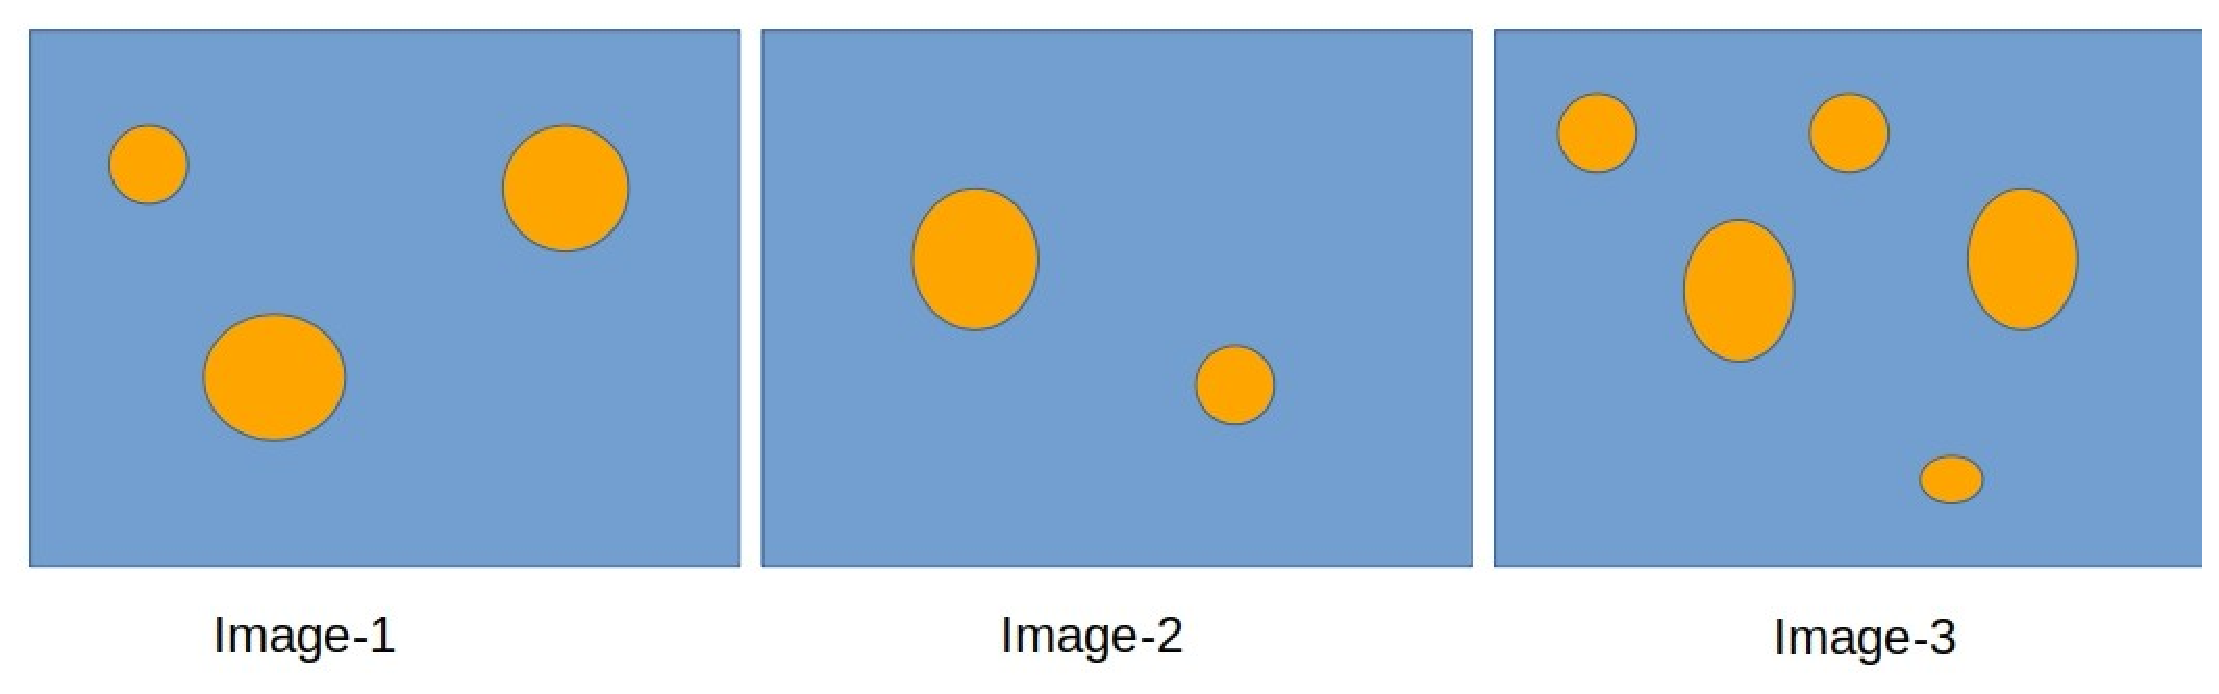
\includegraphics[width=0.75\paperwidth]{question_2/question2.eps} 
\end{center}
\end{figure} 


\subsection{Solution}

Link to the GitHub repository for this question: \href{https://github.com/Xerefic/MM2090-Solutions/tree/master/Final_Assignment/question_2}{GitHub} \footnote{Repo: \url{https://github.com/Xerefic/MM2090-Solutions/tree/master/Final_Assignment/question_2}}

\subsubsection{Approach}
I am using the OpenCV\footnote{\url{https://opencv.org/}} library to pre-process the image – converting it to grayscale, and resizing for uniformity. Followed by applying a binary filter to sort the different colours into just two values – 0 and 255. Basically, every value greater than the minimum pixel value +10 is mapped to 255 and the rest to 0. Given that the image contains only two colours, this process will distinguish the two colours in every case. \\
To count the number of objects, I am using the fact that the gradients across the normal to the contours of the said region is non zero and uniform. findContours identifies continuous boundaries of regions having same colour, where the length of countours gives the number of the objects.


\subsubsection{Requirements}
Language of choice: python
\begin{lstlisting}[language=bash]
	pip3 install numpy	
	pip3 install matplotlib
	pip3 install opencv-python
\end{lstlisting}

\subsubsection{Output}

\begin{table}[!ht]
	\begin{center}
		\begin{tabular}{ | c | p{5cm} | }
			\hline
			IMAGE & PREDICTION \\ \hline
			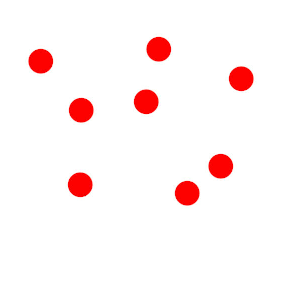
\includegraphics[width=50mm, height=50mm]{question_2/Image-1.eps} & 
				Number of objects = 8 \\ \hline
			
\includegraphics[width=50mm, height=50mm]{question_2/Image-2.eps} &
				Number of objects = 6 \\ \hline
		\end{tabular}
	\end{center}
\caption{Predicted Number of Objects}
\end{table}

\clearpage
\subsection{Code}
\lstinputlisting{question_2/question2.py}